The nonresonant $WW$ contribution in the signal region can be estimated from data 
using the dilepton invariant mass distribution. 
For a given Higgs boson mass, a $\ww$-dominated control region with a small contribution 
from Higgs decays can be selected. The $\ww$ contribution estimated in the control region 
is then extrapolated into the signal region using simulation. 

Figure~\ref{fig:higgsMllCutoff} shows the dilepton invariant mass distributions for 
$\ww$ and $\hww$ with $m_{H} = 130, 200$, and 300~$\GeVcc$. 
For Higgs masses above 200~$\GeVcc$ there is significant overlap in the 
dilepton invariant mass distribution with the nonresonant $\ww$ contribution. 
The control region can not be defined efficiently in that case. Therefore for 
searches for a high mass Higgs ($m_H>200\GeVcc$) we estimate the nonresonant 
$\ww$ contributions from simulation. 

%The basic idea for the estimation of the nonresonant $WW$ contribution in the $\hww$ signal region is 
%to infer it from data using the dilepton mass distribution:
%the dilepton mass defines a control region where we can measure the $WW$ normalization, and then scale
%the contribution to the signal region.

%It turns out that this approach can be applied for $m_H \leq 200~\GeVcc$ only.
%In fact, MC studies show that the di-lepton mass distribution in Higgs samples has a cut-off value at $m_H-50~\GeVcc$ 
%(Fig.~\ref{fig:higgsMllCutoff});
%thus, for large $m_H$ it is possible to define an Higgs-depleted region only in a mass range populated by too 
%few $WW$ events. 

%Therefore, for $m_H > 200~\GeVcc$ the $WW$ contribution is estimated from simulated events.

%%%%%%%%%%%%%%%%%%%%%%%%%%%%%%%%%%%%%%%%%%%
\begin{figure}[!hbtp]
\centering
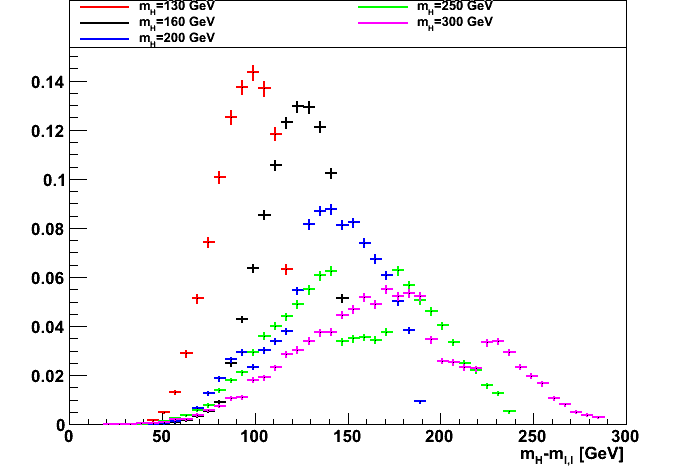
\includegraphics[width=.5\textwidth]{figures/higgsMllCutoff.png}
\caption{The dilepton invariant mass distributions for $\hww$ decays with 
$m_{H} = 130, 200, 300\GeVcc$ in simulation. 
The distributions are normalized to unity.}
\label{fig:higgsMllCutoff}
\end{figure}
%%%%%%%%%%%%%%%%%%%%%%%%%%%%%%%%%%%%%%%%%%%

%\subsubsection{Estimation in Low Mass Range}

For searches for low mass Higgs bosons with $m_{H}<200\GeVcc$, we define the $\ww$ control region as the events 
with $m_{\ell\ell} > 100~\GeVcc$ that pass the full event selection (see Section~\ref{sec:signal_selection}) 
except for the requirements on $m_T$ and $\Delta\phi$. The procedure to obtain the $\ww$ contribution 
in the signal region is as follows. 
%we define the $\ww$ dominated control region dominated by $\ww$ decays as 
%For low Higgs boson mass values ($m_{\rm{H}} \leq 200~\GeVcc$) events with $m_{\ell\ell} > 100~\GeVcc$ are used
%to define a control region where the Higgs contribution is $<3\%$.
\begin{itemize}
\item We first measure the yield in the control region in data; %applying full event selections except for the cuts on 
%$m_{ll}$, 
%$m_T$ and $\Delta\phi_{ll}$% so that most of the systematics uncertainties 
%cancel out (e.g. jet veto, lepton and trigger efficiencies); 
\item We then subtract the contamination from other backgrounds such as $t\bar t$ and $W$+jets (see Table~\ref{tab:wwEstimationSByields}) which can be estimated using corresponding data-driven techniques
\item The resulting yield is subsequently extrapolated to the signal region;
using the control-to-signal region ratio estimated using the dilepton invariant mass spectrum in simulation;
\item Finally, we multiply the yields in the signal region by the 
$m_T$ and $\Delta\phi_{ll}$ cut efficiency from simulation to get the 
$WW$ contribution in the signal region after all cuts.
\end{itemize}

We can validate this procedure by comparing the $m_T$ and $\Delta\phi_{ll}$ cut efficiency 
in the control region between data and simulation with enough statistics. 
Table~\ref{tab:wwEstimationMC} shows the ratio of the $\ww$ contribution in control and 
signal regions referred to as $R_{C/S}$ comparing different MC generators. 
In the 1-jet bin case, we observe a significant discrepancy in the $R_{C/S}$ value between MadGraph and PYTHIA.
Such difference is likely due to the worse description of jet kinematics in the PYTHIA sample. 

\begin{table}[!htbp]
\begin{center}
\begin{tabular}{|c|c|c|c|c|c|} \hline
 sample               &       MuMu &       ElMu &       MuEl &       ElEl &        All \\ \hline\hline
   $qq\rightarrow WW$ &      21.75 &      34.06 &      35.81 &      16.29 &     107.91 \\ 
   $gg\rightarrow WW$ &       0.87 &       1.20 &       1.25 &       0.69 &       4.00 \\ 
  $t\bar t$           &       2.73 &       3.82 &       3.82 &       1.77 &      12.14 \\ 
     tW               &       0.95 &       1.49 &       1.23 &       1.10 &       4.79 \\ 
 W+jets               &       0.00 &       2.08 &       2.08 &       6.24 &      10.40 \\ 
 others               &       2.07 &       0.66 &       0.96 &       1.72 &       5.41 \\ \hline
  total               &      28.36 &      43.31 &      45.16 &      27.81 &     144.64 \\ \hline
\end{tabular}
\caption{Expected yields in the control region from MC (0-jet bin) normalized to an integrated luminosity of $1~fb^{-1}$.}
\label{tab:wwEstimationSByields}
\end{center}
\end{table}

\begin{table}[!htbp]
\begin{center}
\begin{tabular}{|c|c|c|} \hline
\multicolumn{3}{|c|}{0-jet bin} \\ \hline
quantity                           &             MadGraph &              PYTHIA  \\ \hline
$R_{C/S}$                           &      0.294$\pm$ 0.005&      0.271$\pm$ 0.011\\
$\epsilon_{m_T}$(mass region)       &      0.877$\pm$ 0.018&      0.877$\pm$ 0.046\\
$\epsilon_{\Delta\phi}$(mass region) &      0.657$\pm$ 0.015&      0.645$\pm$ 0.040\\
$\epsilon_{m_T}$(side band)         &      0.544$\pm$ 0.007&      0.544$\pm$ 0.017\\
$\epsilon_{\Delta\phi}$(side band)   &      0.051$\pm$ 0.002&      0.036$\pm$ 0.005\\ \hline \hline
\multicolumn{3}{|c|}{1-jet bin} \\ \hline
quantity                           &             MadGraph &              PYTHIA  \\ \hline
$R_{C/S}$                           &    0.320$\pm$ 0.008 &      0.221$\pm$ 0.018 \\
$\epsilon_{m_T}$(mass region)       &    0.759$\pm$ 0.026 &      0.737$\pm$ 0.086 \\
$\epsilon_{\Delta\phi}$(mass region) &   0.814$\pm$ 0.031 &      0.775$\pm$ 0.103  \\
$\epsilon_{m_T}$(side band)         &    0.521$\pm$ 0.011 &      0.513$\pm$ 0.031 \\
$\epsilon_{\Delta\phi}$(side band)   &   0.105$\pm$ 0.006 &      0.086$\pm$ 0.015  \\ \hline
\end{tabular}
\caption{Control-to-signal region ratio and cut efficiencies using MadGraph $qq\rightarrow WW$ and PYTHIA $gg\rightarrow WW$
vs PYTHIA inclusive $WW$. Results for $m_H=160~\GeVcc$ analysis in the 0- and 1-jet bins. 
Uncertainties are statistical only and account for the MC sample luminosity. }
\label{tab:wwEstimationMC}
\end{center}
\end{table}

We perform a closure test of this procedure on simulation events. In this test we mix the events from 
$\WW$ (including $qq\rightarrow WW$ and $gg\rightarrow WW$), $t\bar t$ and $tW$ according to their SM cross-sections 
normalized to an integrated luminosity of $1~\text{fb}^{-1}$ to approximate the data composition. 
The $qq\rightarrow WW$ events are taken from PYTHIA while the rest are taken from Madgraph. 
%For the moment we consider only the main contamination source in the side band region, top background; 
The expected yields of $\ww$ and top backgrounds in the control region % relaxing the $m_{T}$ and $\Delta\phi$ cuts  
are 111.9 and 16.9 respectively (see Table~\ref{tab:wwEstimationSByields}). 
Based on this mixed simulation data, we apply the $\ww$ background estimation method described above. 
The top contribution is estimated as 10.5$\pm$4.1 events with the data-driven method (Section~\ref{sec:bkg_top}) 
using the top tagging efficiency in a top-enriched sample. 
The $R_{C/S}$ ratio and selection efficiencies of $m_T$ and $\Delta\phi$ cuts evaluated in the inclusive PYTHIA MC 
are then 
used to estimate the $\ww$ contribution in the Higgs signal region. 
%Therefore, we estimate 118.4$\pm$12.1 $WW$ events in the side band region and, after applying
%the control-to-signal region ratio and the cut efficiencies, 18.2$\pm$2.3 events in the $m_H=160~\GeVcc$ signal region 
%(consistent with the expected value of 18.9$\pm$0.3).
Results for all considered Higgs masses in the 0- and 1-jet bins are reported in Table~\ref{tab:wwEstimationRes}.
The agreement in the 0-jet bin is very good, while in the 1-jet bins there are $\sim1\sigma$ discrepancies due to the underestimated 
PYTHIA $R_{C/S}$ value.

\begin{table}[!htbp]
\begin{center}
\begin{tabular}{|c|c|c|} \hline
\multicolumn{3}{|c|}{0-jet bin} \\ \hline
$m_H~[\GeVcc]$ & WW estimation ($1~fb^{-1}$) & WW expected ($1~fb^{-1}$)  \\ \hline
120 & 41.2 $\pm$ 4.9 & 43.4 $\pm$ 0.5 \\
130 & 45.4 $\pm$ 5.2 & 47.4 $\pm$ 0.5 \\
140 & 41.7 $\pm$ 4.9 & 42.7 $\pm$ 0.5 \\
150 & 28.3 $\pm$ 3.7 & 28.4 $\pm$ 0.4 \\
160 & 18.2 $\pm$ 2.5 & 18.9 $\pm$ 0.3 \\
200 & 11.7 $\pm$ 1.6 & 12.2 $\pm$ 0.3 \\ \hline \hline
\multicolumn{3}{|c|}{1-jet bin} \\ \hline
$m_H~[\GeVcc]$ & WW estimation ($1~fb^{-1}$) & WW expected ($1~fb^{-1}$)  \\ \hline
120 & 6.2 $\pm$ 4.6 & 9.6 $\pm$ 0.2 \\
130 & 6.8 $\pm$ 5.1 & 10.7$\pm$ 0.2 \\
140 & 6.3 $\pm$ 4.7 & 9.7 $\pm$ 0.2 \\
150 & 4.6 $\pm$ 3.8 & 8.9 $\pm$ 0.2 \\
160 & 3.6 $\pm$ 3.0 & 7.4 $\pm$ 0.2 \\
200 & 4.4 $\pm$ 3.7 & 8.8 $\pm$ 0.2 \\
 \hline
\end{tabular}
\caption{Closure test result of $WW$ estimation for different Higgs mass analyses in the 0- and 1-jet bins.  
Errors are statistical only; in the WW estimation column they are computed for a luminosity of $1~fb^{-1}$, 
while in the WW expected column they correspond to the MC sample luminosity.}
\label{tab:wwEstimationRes}
\end{center}
\end{table}


%Systematics are evaluated repeating the procedure varying the usual suspects.

%
%\subsection{Estimation in high mass range}
%We take it from MC.



%The nonresonant $qq \to \WW$ contribution in the $\hww$ signal region is 
%estimated from data using the dilepton mass distribution. For a given Higgs 
%boson mass, the region with a small contribution from Higgs boson decays is 
%selected and simulation is used to extrapolate this background into the signal 
%region. For low Higgs boson mass values ($m_{\rm{H}} < 200~\GeVcc$) events 
%with $m_{\ell\ell} > 100~\GeVcc$ are used, while for $m_{\rm{H}} > 200~\GeVcc$ 
%events with $m_{\ell\ell} < 100~\GeVcc$ are used. The statistical uncertainty 
%on the estimate of the nonresonant $\WW$ background with the current data 
%sample is approximately 50\%. For the 1- and 2- jet bin cases we use the results
%from the 0-jet bin, and then extrapolate to each jet bin.
%
%The $gg \to \WW$ background contribution has to be taken from simulated events 
%since we do not have enough sensitivity in the data to measure it. We assign a 
%50\% uncertainty to the overall normalization~\cite{ggWWError}. This is 
%obtained by studying the change in the cross-section when varying the parton 
%distribution functions (PDFs), QCD renormalization and scales.
